% ─────────────────────────────────────────────────────────────────────────────
This chapter provides the important design artifacts for the BookForMe project,
covering the software architecture, data model, agentic pipeline, key algorithms,
and workflow diagrams.

% ─────────────────────────────────────────────────────────────────────────────
\section{Software Design}
\label{sec:sds-design}

\subsection{Architectural Overview}

BookForMe follows a \textbf{Service-Oriented Architecture (SOA)} with a strict
separation between the Presentation, Business Logic, and Persistence layers.  The
architecture supports two distinct client types:

\begin{enumerate}
  \item \textbf{Rich Client (Mobile App):} Connects via HTTPS / JSON.  Best for
        power users who want to browse categories, manage a profile, and join
        social lobbies.
  \item \textbf{Conversational Client (WhatsApp):} Connects via Webhooks to the AI
        Receptionist.  Best for quick bookings without installing an app, using
        natural language in English or Roman Urdu.
\end{enumerate}

Both clients converge on a single backend and Firestore database---the
\textbf{Single Source of Truth}---ensuring that a booking made via WhatsApp is
immediately reflected in the mobile app and on the vendor dashboard.  The Central
Backend API is the sole orchestrator; it delegates to the AI Agent and OCR Service
for specialised logic.  Dependencies are strictly unidirectional: Clients depend on
Backend; Backend depends on Database.

\begin{figure}[H]
  \centering
  \IfFileExists{images/System Architecture.png}{
    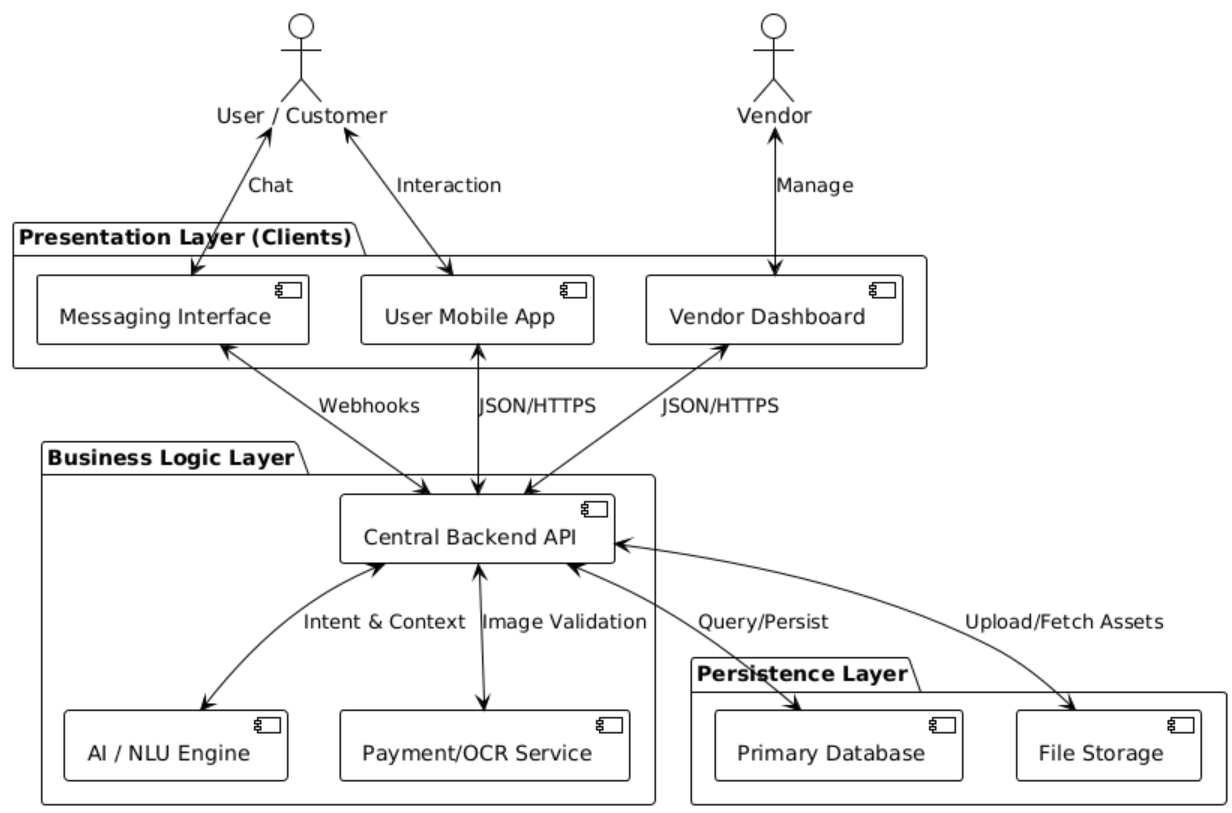
\includegraphics[width=0.95\textwidth]{images/System Architecture.png}
  }{
    \fbox{\parbox{0.85\textwidth}{\centering\vspace{0.8cm}
    Missing figure file: \texttt{images/System Architecture.png}\par
    System architecture diagram placeholder\vspace{0.8cm}}}
  }
  \caption{Primary system architecture of BookForMe.}
  \label{fig:sds-system-architecture}
\end{figure}

\begin{figure}[H]
  \centering
  \IfFileExists{images/system-overview.png}{
    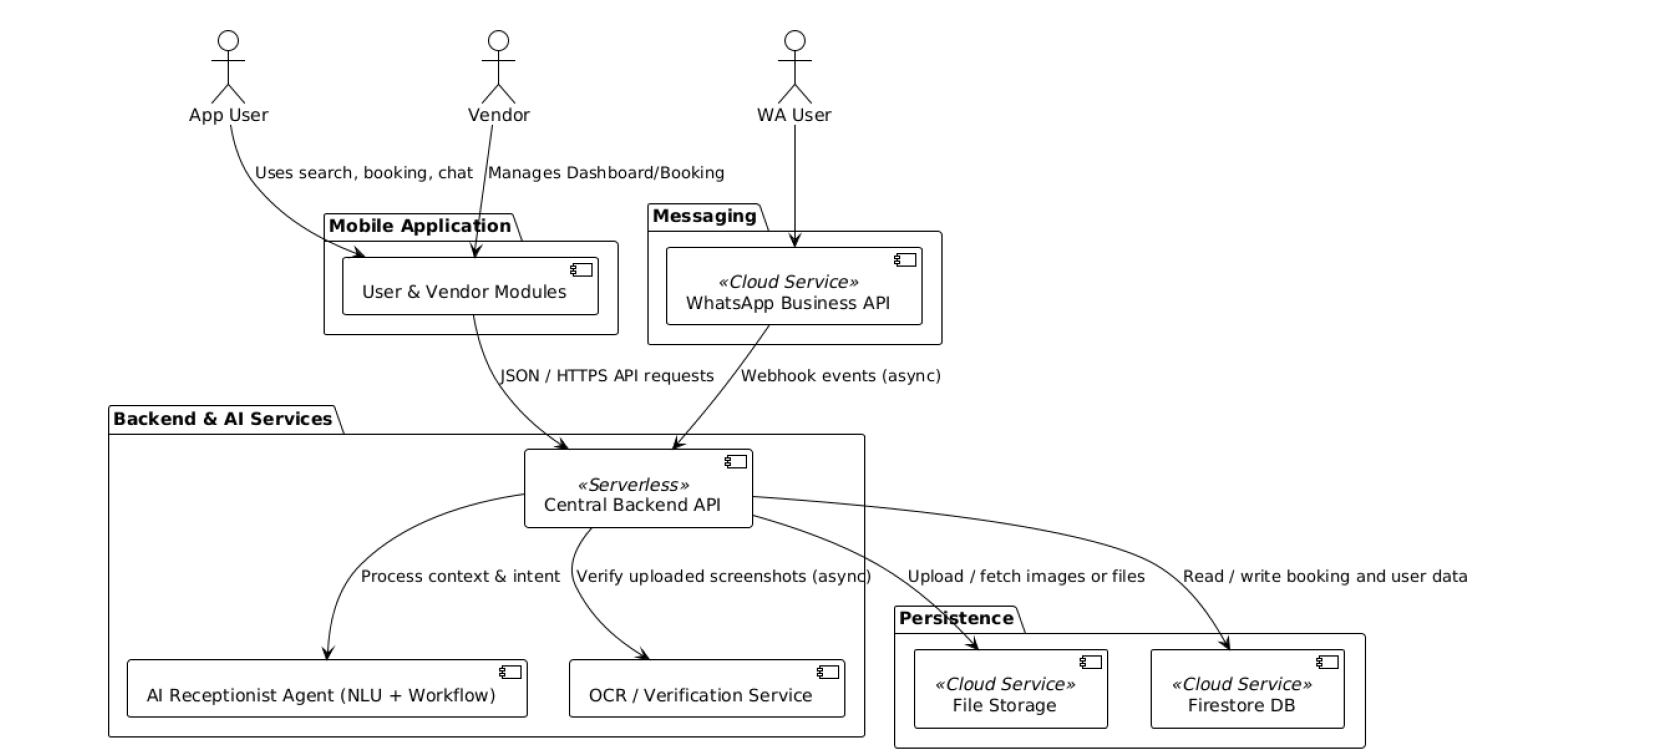
\includegraphics[width=0.95\textwidth]{images/system-overview.png}
  }{
    \fbox{\parbox{0.85\textwidth}{\centering\vspace{0.8cm}
    Missing figure file: \texttt{images/system-overview.png}\par
    System overview diagram placeholder\vspace{0.8cm}}}
  }
  \caption{System overview showing major platform components.}
  \label{fig:sds-system-overview}
\end{figure}

\subsection{Architectural Design Decisions}

\begin{description}
  \item[Neuro-Symbolic AI Architecture]
        The LLM (Gemini) interprets natural language (creative / linguistic),
        but all database mutations are executed by deterministic LangGraph code nodes
        (symbolic / strict logic).  This prevents the agent from ``hallucinating''
        bookings or bypassing payment requirements.  It also provides a natural
        security boundary against prompt-injection attacks.

  \item[Cyclic State Graph (LangGraph)]
        Unlike linear DAG-based pipelines, the LangGraph cyclic state graph can loop
        back---e.g., returning to ``Classify Intent'' after receiving a corrected
        payment screenshot.  This is essential for WhatsApp's asynchronous,
        multi-turn nature.

  \item[Reference-Based NoSQL Schema]
        Firestore's document model is used with a Reference-Based strategy: entities
        store document references (IDs) rather than embedding full sub-documents.
        This balances NoSQL flexibility with structured relational integrity and
        avoids document-size limits.

  \item[Strict Social / Transactional Separation]
        The Firestore schema separates the \textbf{Social Ecosystem} (user reputation,
        matchmaking, forums) from the \textbf{Transactional Domain} (vendors,
        services, bookings, payments).  High-volume social interactions cannot
        degrade the performance or integrity of critical financial data.
\end{description}

\begin{figure}[H]
  \centering
  \IfFileExists{images/FYP - SAD.png}{
    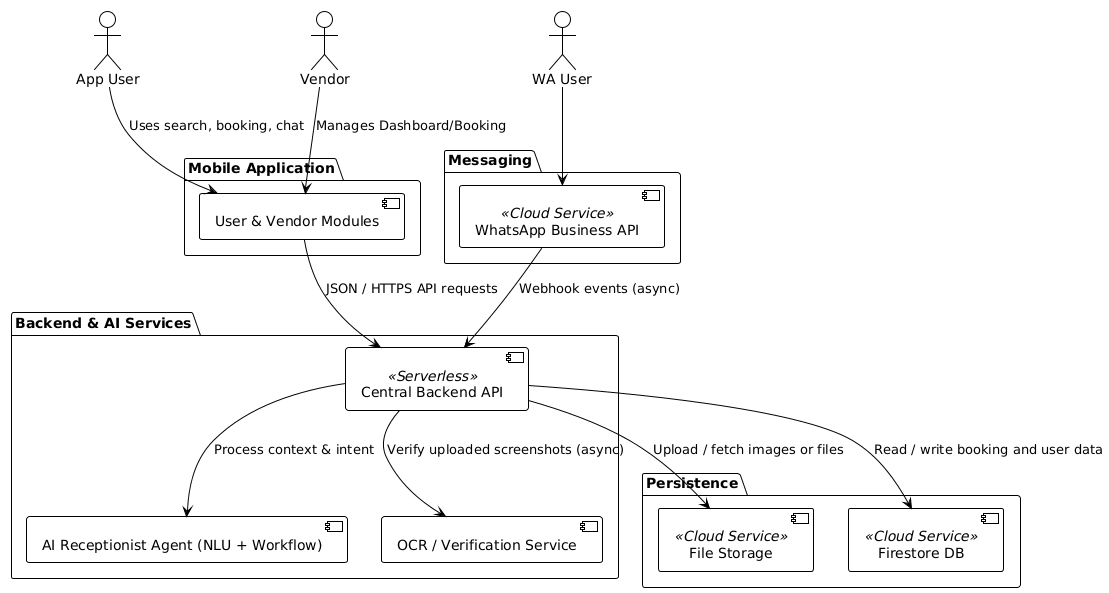
\includegraphics[width=0.95\textwidth]{images/FYP - SAD.png}
  }{
    \fbox{\parbox{0.85\textwidth}{\centering\vspace{0.8cm}
    Missing figure file: \texttt{images/FYP - SAD.png}\par
    Software architecture diagram placeholder\vspace{0.8cm}}}
  }
  \caption{Software Architecture Diagram (SAD) for BookForMe.}
  \label{fig:sds-fyp-sad}
\end{figure}

% ─────────────────────────────────────────────────────────────────────────────
\section{Data Design}
\label{sec:sds-data}

\subsection{Database Strategy}

Data persistence is handled by \textbf{Google Cloud Firestore}, a serverless NoSQL
document database.  The schema is divided into two domains:

\begin{itemize}
  \item \textbf{User \& Social Domain:} Manages user engagement (reputation,
        matchmaking, friends, forums, DMs) without affecting financial data integrity.
  \item \textbf{Core Booking Domain:} Manages all business logic (vendors, services,
        bookings, payments) with strong consistency guarantees via Firestore
        transactions.
\end{itemize}

\subsection{Entity Descriptions}

Table~\ref{tab:entities} describes the primary data entities and their roles.

\begin{table}[H]
\centering
\caption{Domain entity descriptions.}
\label{tab:entities}
\small
\begin{tabularx}{\textwidth}{>{\raggedright\arraybackslash}p{0.20\textwidth}Y Y}
\toprule
\textbf{Entity} & \textbf{Key Attributes} & \textbf{Description} \\
\midrule
\texttt{Users}
  & \texttt{user\_id}, \texttt{auth\_uid},
    \texttt{elo\_rating}, \texttt{skill\_profile}
  & Central anchor bridging social features (Elo ratings) and commercial features
    (booking history). \\[4pt]
\texttt{Vendors}
  & \texttt{vendor\_id}, \texttt{location\_geo},
    \texttt{category}, \texttt{owner\_ref}
  & Business entity defined independently of services to support scalable inventory
    management. \\[4pt]
\texttt{Services}
  & \texttt{service\_id}, \texttt{vendor\_ref},
    \texttt{price\_per\_slot}, \texttt{type}
  & The sellable unit (e.g., a specific Futsal Court or Gaming PC). \\[4pt]
\texttt{Bookings}
  & \texttt{booking\_id}, \texttt{user\_ref},
    \texttt{service\_ref}, \texttt{hold\_expires\_at},
    \texttt{status}, \texttt{payment\_ref}
  & Transactional record.  Includes \texttt{hold\_expires\_at} timestamp for OCC
    slot locking.  Status: \{HOLD, PENDING\_APPROVAL, CONFIRMED, REJECTED\}. \\[4pt]
\texttt{Payments}
  & \texttt{transaction\_id}, \texttt{screenshot\_url},
    \texttt{ocr\_verified\_amount}, \texttt{status}
  & Separated from \texttt{Bookings} for auditability.  Stores raw screenshot and
    OCR-validated amount.  Status: \{PENDING, VERIFIED, REJECTED\}. \\[4pt]
\texttt{Match\_Lobbies}
  & \texttt{match\_id}, \texttt{host\_ref},
    \texttt{participants}, \texttt{mode},
    \texttt{avg\_elo}, \texttt{status}
  & Manages matchmaking queues for Ranked and Casual lobbies. \\[4pt]
\texttt{Forum\_Posts}
  & \texttt{post\_id}, \texttt{author\_ref},
    \texttt{content}, \texttt{timestamp},
    \texttt{comments} (sub-collection)
  & Community posts driving social engagement. \\[4pt]
\texttt{Direct\_Messages}
  & \texttt{chat\_id}, \texttt{participants},
    \texttt{last\_message}, \texttt{last\_timestamp}
  & Peer-to-peer chat between users on the friends list. \\
\bottomrule
\end{tabularx}
\end{table}

\begin{figure}[H]
  \centering
  \IfFileExists{images/ERD.png}{
    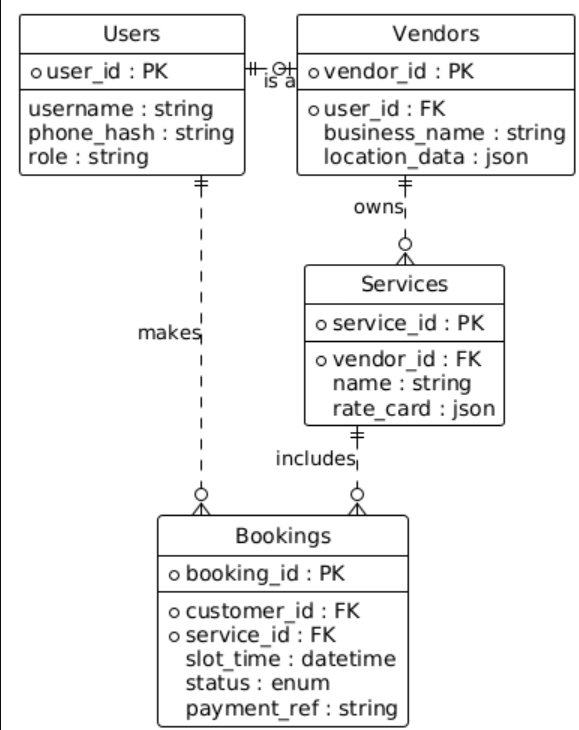
\includegraphics[width=0.95\textwidth]{images/ERD.png}
  }{
    \fbox{\parbox{0.85\textwidth}{\centering\vspace{0.8cm}
    Missing figure file: \texttt{images/ERD.png}\par
    ERD placeholder\vspace{0.8cm}}}
  }
  \caption{Entity Relationship Diagram (ERD) for the core data model.}
  \label{fig:sds-erd}
\end{figure}

\begin{figure}[H]
  \centering
  \IfFileExists{images/Data Model.png}{
    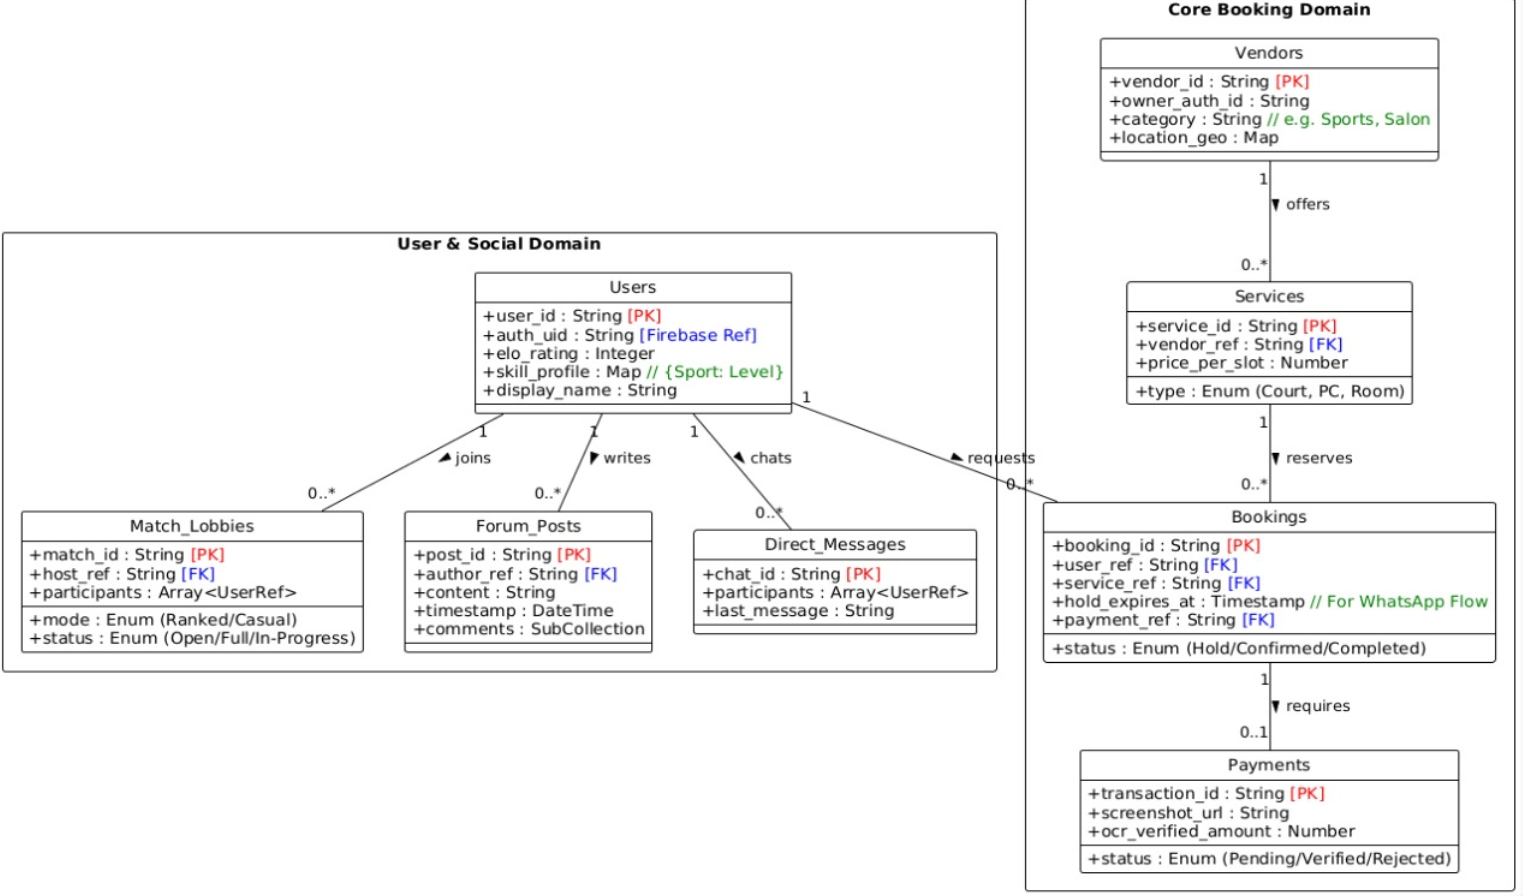
\includegraphics[width=0.95\textwidth]{images/Data Model.png}
  }{
    \fbox{\parbox{0.85\textwidth}{\centering\vspace{0.8cm}
    Missing figure file: \texttt{images/Data Model.png}\par
    Data model placeholder\vspace{0.8cm}}}
  }
  \caption{Detailed data model used for Firestore document structure.}
  \label{fig:sds-data-model}
\end{figure}

\begin{figure}[H]
  \centering
  \IfFileExists{images/Class diagram.png}{
    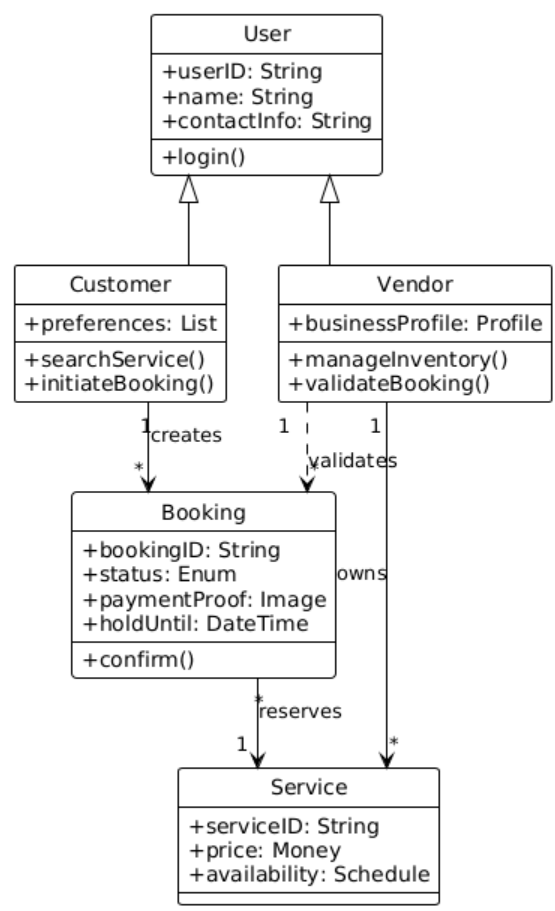
\includegraphics[width=0.95\textwidth]{images/Class diagram.png}
  }{
    \fbox{\parbox{0.85\textwidth}{\centering\vspace{0.8cm}
    Missing figure file: \texttt{images/Class diagram.png}\par
    Class diagram placeholder\vspace{0.8cm}}}
  }
  \caption{Class diagram for major domain objects and relationships.}
  \label{fig:sds-class-diagram}
\end{figure}

\subsection{Booking Status Lifecycle}

Figure~\ref{fig:booking-lifecycle} shows the state machine for a booking record.

\begin{figure}[H]
  \centering
  \IfFileExists{images/AD- App flow booking process.png}{
    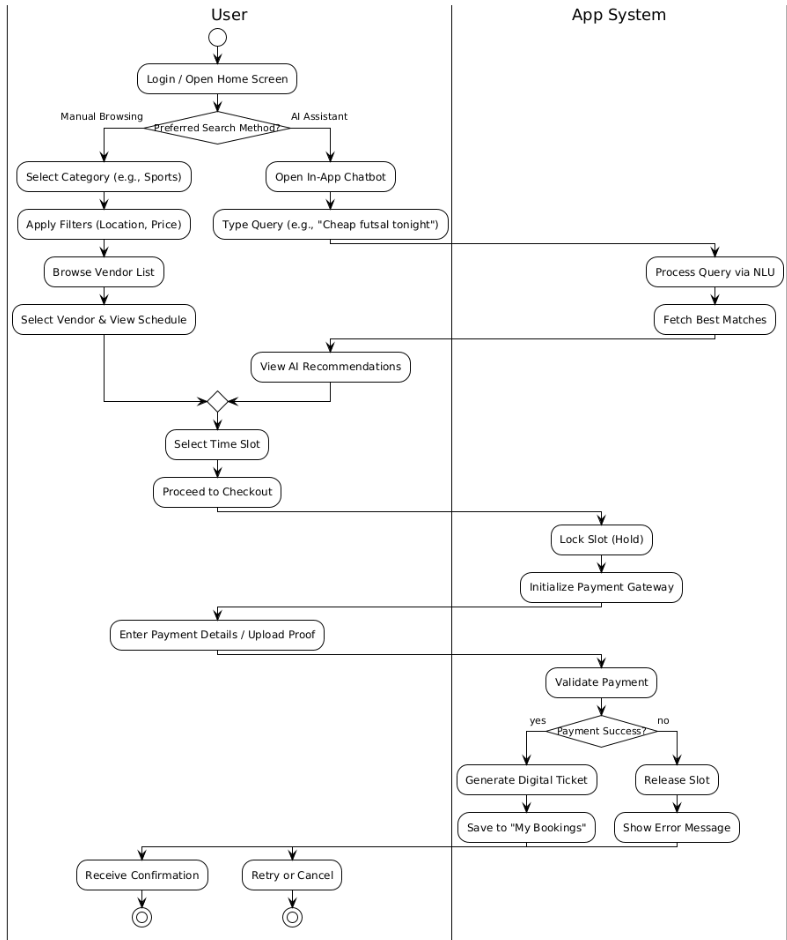
\includegraphics[width=0.95\textwidth]{images/AD- App flow booking process.png}
  }{
    \fbox{\parbox{0.85\textwidth}{\centering\vspace{0.8cm}
    Missing figure file: \texttt{images/AD- App flow booking process.png}\par
    Booking lifecycle state machine placeholder\vspace{0.8cm}}}
  }
  \caption{Booking record state lifecycle.}
  \label{fig:booking-lifecycle}
\end{figure}

% ─────────────────────────────────────────────────────────────────────────────
\section{Technical Details}
\label{sec:sds-technical}

\subsection{Key Algorithms}

\subsubsection{Algorithm 1: Intent Parsing and Action Routing}

\textbf{Purpose:} Translate unstructured natural language into deterministic
database actions without hallucination.

\textbf{Input:} Raw WhatsApp message string + serialised user session state.

\textbf{Logic:}
\begin{enumerate}
  \item The fine-tuned DistilBERT model classifies the user's message into one of
        five intent classes: \texttt{inquiry}, \texttt{info},
        \texttt{transaction\_confirm}, \texttt{greeting}, \texttt{unknown}.
  \item The Gemini API (fallback for complex or ambiguous cases) extracts slot
        entities: service type, date, time, duration, budget, location.
  \item The classified intent routes to a specific LangGraph node which executes
        rigid Python code (e.g., a Firestore query) rather than allowing the LLM
        to generate queries itself.
  \item If required slots are missing, the Validate State node generates a targeted
        clarification question and loops back to Classify Intent.
\end{enumerate}

\textbf{Output:} Validated JSON payload routed to the appropriate action node,
or a clarification prompt sent back to the user.

\subsubsection{Algorithm 2: Optimistic Concurrency Control (OCC)}

\textbf{Purpose:} Prevent race conditions (double-bookings) in the distributed
Firestore environment.

\textbf{Input:} \texttt{service\_id}, \texttt{time\_slot}, \texttt{user\_id}.

\textbf{Logic:}
\begin{enumerate}
  \item \textbf{Read:} Fetch the current document for the requested time slot.
  \item \textbf{Verify:} Check that \texttt{status == "AVAILABLE"} and that no
        unexpired HOLD exists (\texttt{hold\_expires\_at > now()}).
  \item \textbf{Write (Atomic):} Within a Firestore transaction, update
        \texttt{status} to \texttt{"HOLD"} and set \texttt{hold\_expires\_at} to
        \texttt{now() + 10 minutes}.  This atomic write automatically fails if the
        underlying document was modified since the Read step.
  \item \textbf{On conflict:} Query the next three available slots from the same
        vendor and offer them to the user as alternatives.
\end{enumerate}

\textbf{Output:} Transaction success with \texttt{booking\_id}, or a conflict error
triggering the alternative-slot flow.

\subsubsection{Algorithm 3: Elo-Based Matchmaking}

\textbf{Purpose:} Pair users of similar skill level for Ranked sport matches.

\textbf{Input:} User's current Elo rating $R_u$, preferred sport, accumulated
wait time $t$.

\textbf{Logic:}
\begin{enumerate}
  \item Compute the search window: $\Delta = 200 + 50 \cdot \lfloor t/60 \rfloor$
        (expands by 50 points for every additional minute waiting).
  \item Query \texttt{Match\_Lobbies} collection for open lobbies of the same sport
        where $|R_u - \text{avg\_elo}| \leq \Delta$ and
        \texttt{status == "Open"}.
  \item If a lobby is found, add the user to \texttt{participants} and check if the
        lobby is now full; if full, transition to \texttt{"In-Progress"}.
  \item If no lobby is found, create a new lobby with \texttt{avg\_elo = R\_u}.
\end{enumerate}

\textbf{Output:} \texttt{lobby\_id} for an existing or newly created lobby, or a
WAIT signal if the user is the first in a new lobby.

\subsubsection{Algorithm 4: Elo Rating Update}

After a ranked match completes, both players' ratings are updated using the standard
Elo formula:

\begin{equation}
  R' = R + K \cdot (S - E)
  \label{eq:elo}
\end{equation}

\noindent where $R$ is the current rating, $K = 32$ is the development coefficient,
$S \in \{0, 0.5, 1\}$ is the actual score (loss/draw/win), and:
\begin{equation}
  E = \frac{1}{1 + 10^{(R_{\text{opp}} - R)/400}}
  \label{eq:elo-expected}
\end{equation}
is the expected score against an opponent with rating $R_{\text{opp}}$~\cite{elo1978}.

\subsection{The LangGraph Agent State Machine}

Figure~\ref{fig:langgraph} illustrates the full LangGraph node graph for the AI
Receptionist.

\begin{figure}[H]
  \centering
  \IfFileExists{images/sds/langgraph-state-machine.png}{
    \includegraphics[width=0.9\textwidth]{images/sds/langgraph-state-machine.png}
  }{
    \fbox{\parbox{0.85\textwidth}{\centering\vspace{0.8cm}
    Missing figure file: \texttt{images/sds/langgraph-state-machine.png}\par
    LangGraph state machine placeholder\vspace{0.8cm}}}
  }
  \caption{LangGraph cyclic state graph for the AI Receptionist.}
  \label{fig:langgraph}
\end{figure}

\subsection{Workflow Visualisations}

\subsubsection{Workflow 1: The Agentic (WhatsApp) Booking Experience}

The agentic booking pipeline proceeds through four phases:

\begin{description}
  \item[Phase 0 --- Natural Language Negotiation]
        The agent maintains a conversational loop, extracting booking intent and all
        required slot entities (service, date, time, budget, location) before querying
        the database.  Incomplete requests trigger clarification prompts in the user's
        preferred language.

  \item[Phase 1 --- Concurrency Lock]
        Once intent is finalised, an atomic Firestore transaction creates a HOLD
        booking with a 10-minute \texttt{hold\_expires\_at}.  Concurrent conflicting
        requests fail at this transaction and receive alternative slot suggestions.

  \item[Phase 2 --- Intelligent Payment Verification]
        The agent requests a payment screenshot (advance payment = 50\% of total).
        The OCR service extracts the amount.  If it does not match, the system
        auto-rejects and re-prompts without alerting the vendor.  This loop continues
        until a valid screenshot is received.

  \item[Phase 3 --- Human-in-the-Loop Vendor Approval]
        Only validated payment records are forwarded to the Vendor Dashboard as push
        notifications.  The vendor reviews the booking and payment proof and approves
        or rejects.  Approval sends the user a confirmation ticket; rejection releases
        the held slot.
\end{description}

\begin{figure}[H]
  \centering
  \IfFileExists{images/Activity Diagram- Whatsapp Booking flow.png}{
    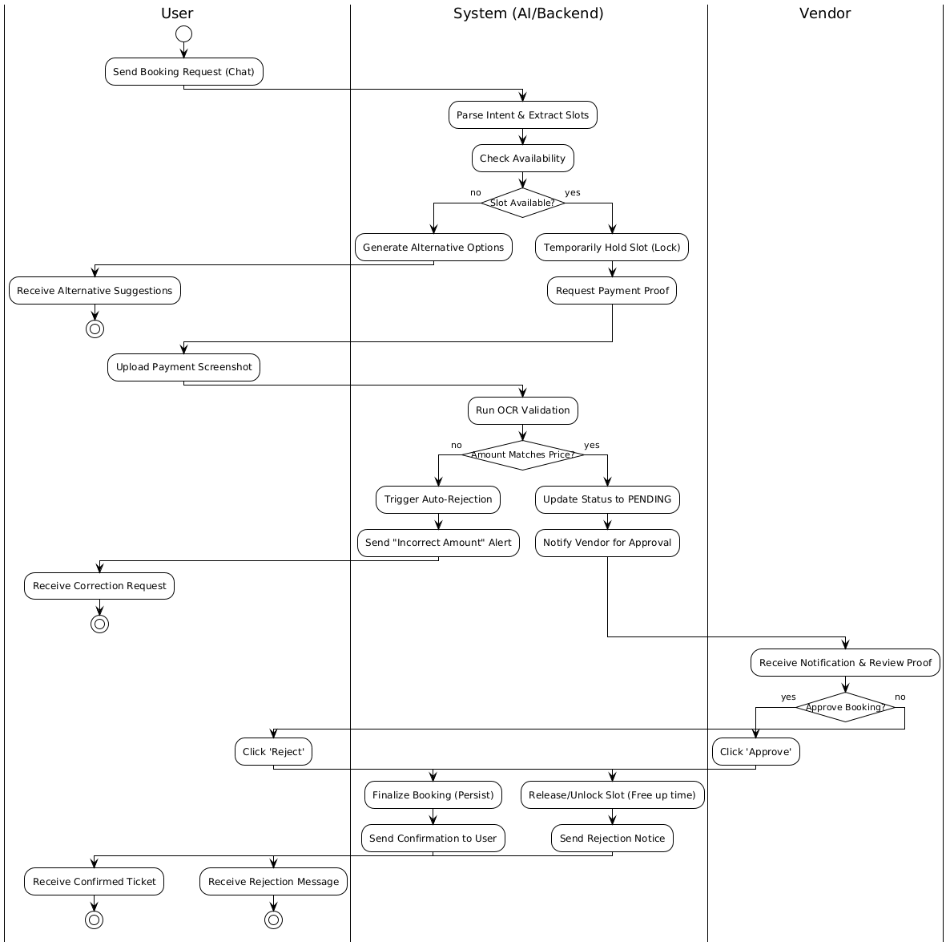
\includegraphics[width=0.95\textwidth]{images/Activity Diagram- Whatsapp Booking flow.png}
  }{
    \fbox{\parbox{0.85\textwidth}{\centering\vspace{0.8cm}
    Missing figure file: \texttt{images/Activity Diagram- Whatsapp Booking flow.png}\par
    WhatsApp booking activity diagram placeholder\vspace{0.8cm}}}
  }
  \caption{Activity diagram of the WhatsApp booking flow.}
  \label{fig:sds-whatsapp-activity}
\end{figure}

\begin{figure}[H]
  \centering
  \IfFileExists{images/FYP - Seq Dig.png}{
    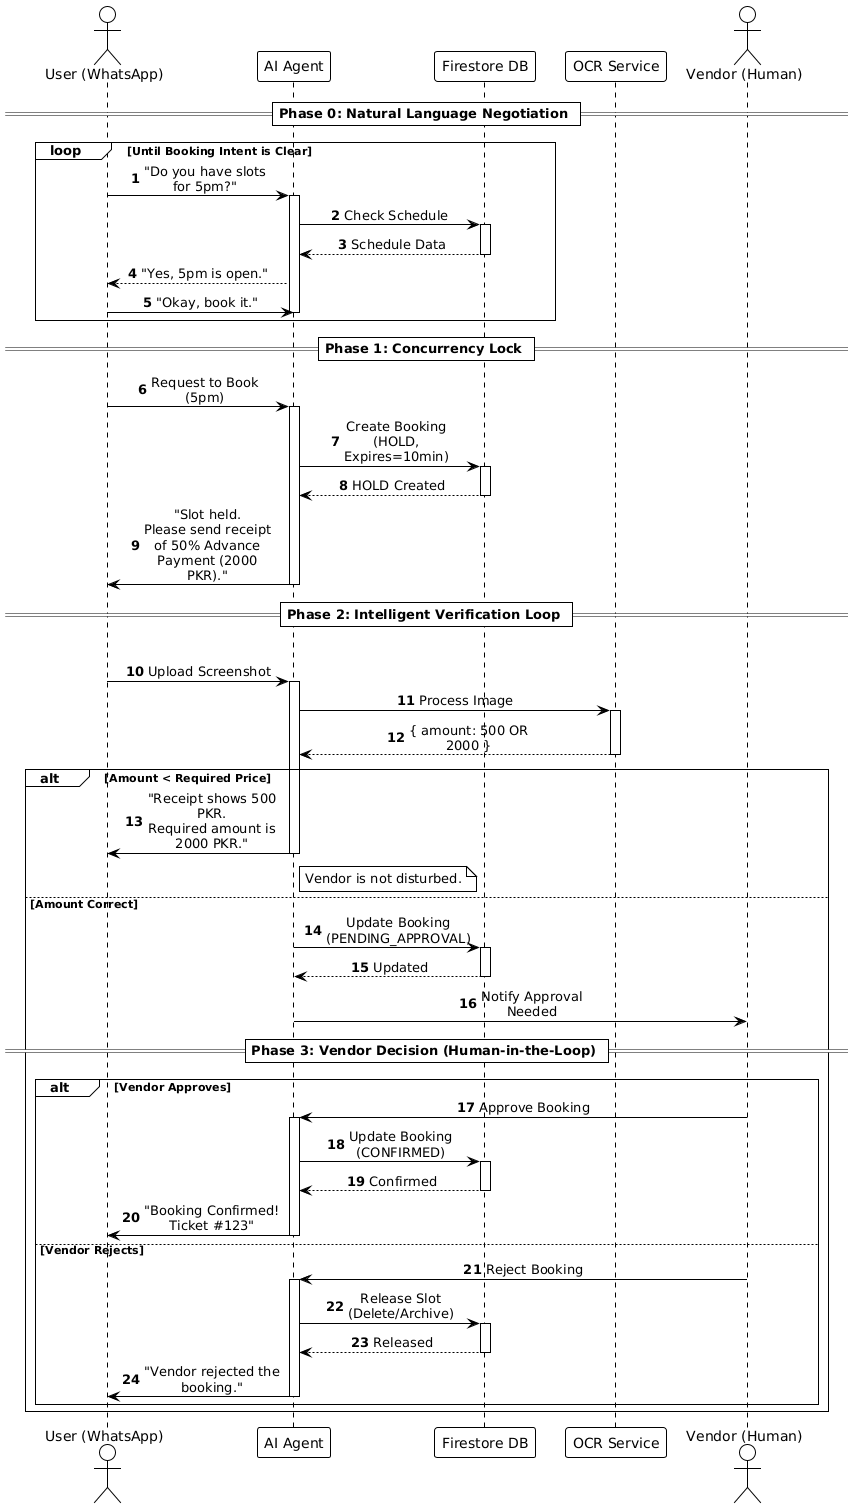
\includegraphics[width=0.95\textwidth]{images/FYP - Seq Dig.png}
  }{
    \fbox{\parbox{0.85\textwidth}{\centering\vspace{0.8cm}
    Missing figure file: \texttt{images/FYP - Seq Dig.png}\par
    Sequence diagram placeholder\vspace{0.8cm}}}
  }
  \caption{Sequence diagram for the agentic booking interaction.}
  \label{fig:sds-seq-whatsapp}
\end{figure}

\begin{figure}[H]
  \centering
  \IfFileExists{images/FYP - Seq Dig (1).png}{
    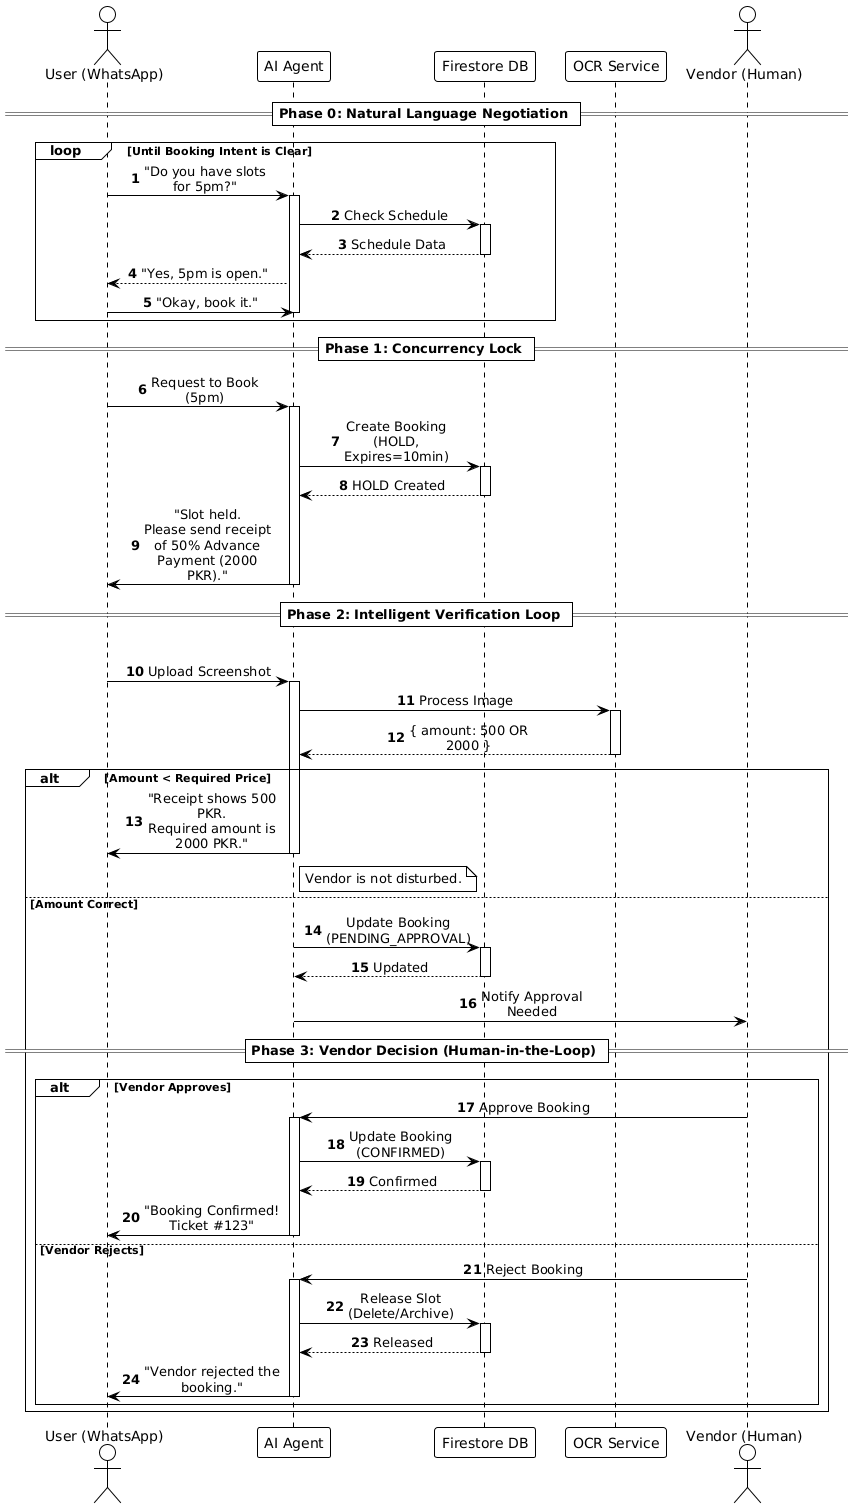
\includegraphics[width=0.95\textwidth]{images/FYP - Seq Dig (1).png}
  }{
    \fbox{\parbox{0.85\textwidth}{\centering\vspace{0.8cm}
    Missing figure file: \texttt{images/FYP - Seq Dig (1).png}\par
    Sequence diagram variant placeholder\vspace{0.8cm}}}
  }
  \caption{Sequence diagram variant covering alternate message flow.}
  \label{fig:sds-seq-whatsapp-alt}
\end{figure}

\subsubsection{Workflow 2: The App User Experience}

A key design feature is the \textbf{Dual-Search Capability}: users can either (a)
browse vendors manually using category and filter screens, or (b) open the embedded
AI Chatbot and type a natural-language query (e.g., ``Cheap futsal tonight in DHA'').
The chatbot uses the same NLU pipeline as the WhatsApp agent to process queries and
returns matching vendor cards.  Both paths converge on the same slot-selection,
checkout, and payment-upload flow.

\begin{figure}[H]
  \centering
  \IfFileExists{images/AD- App flow booking process.png}{
    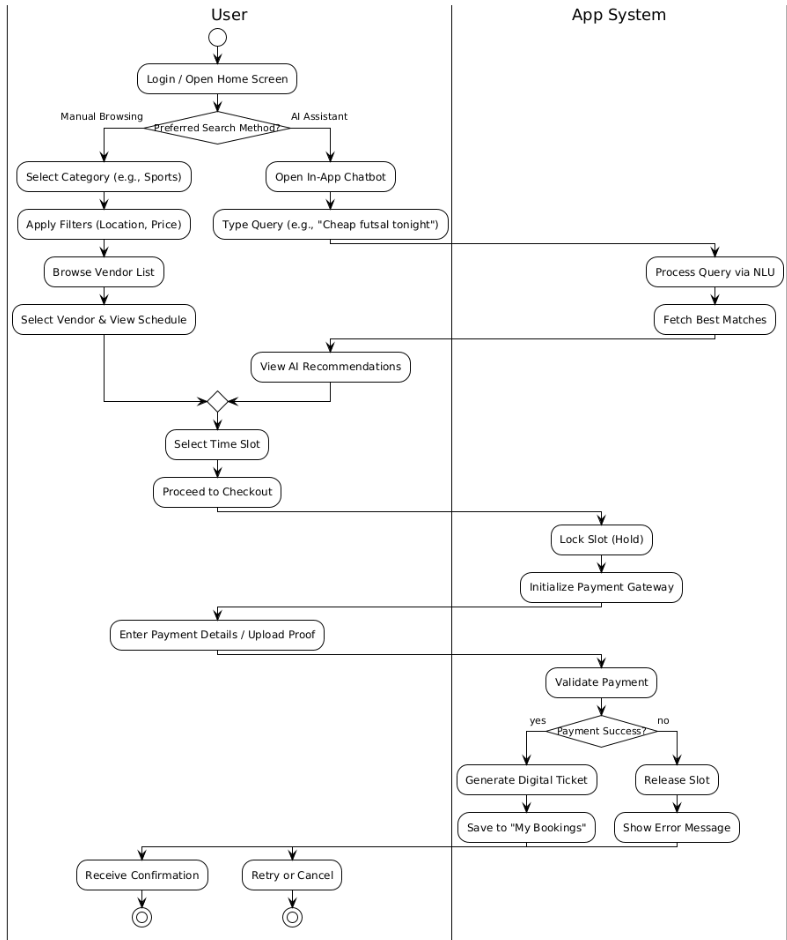
\includegraphics[width=0.95\textwidth]{images/AD- App flow booking process.png}
  }{
    \fbox{\parbox{0.85\textwidth}{\centering\vspace{0.8cm}
    Missing figure file: \texttt{images/AD- App flow booking process.png}\par
    App flow activity diagram placeholder\vspace{0.8cm}}}
  }
  \caption{Activity diagram for the in-app booking process.}
  \label{fig:sds-app-booking-activity}
\end{figure}

\begin{figure}[H]
  \centering
  \IfFileExists{images/Activity Diagram.png}{
    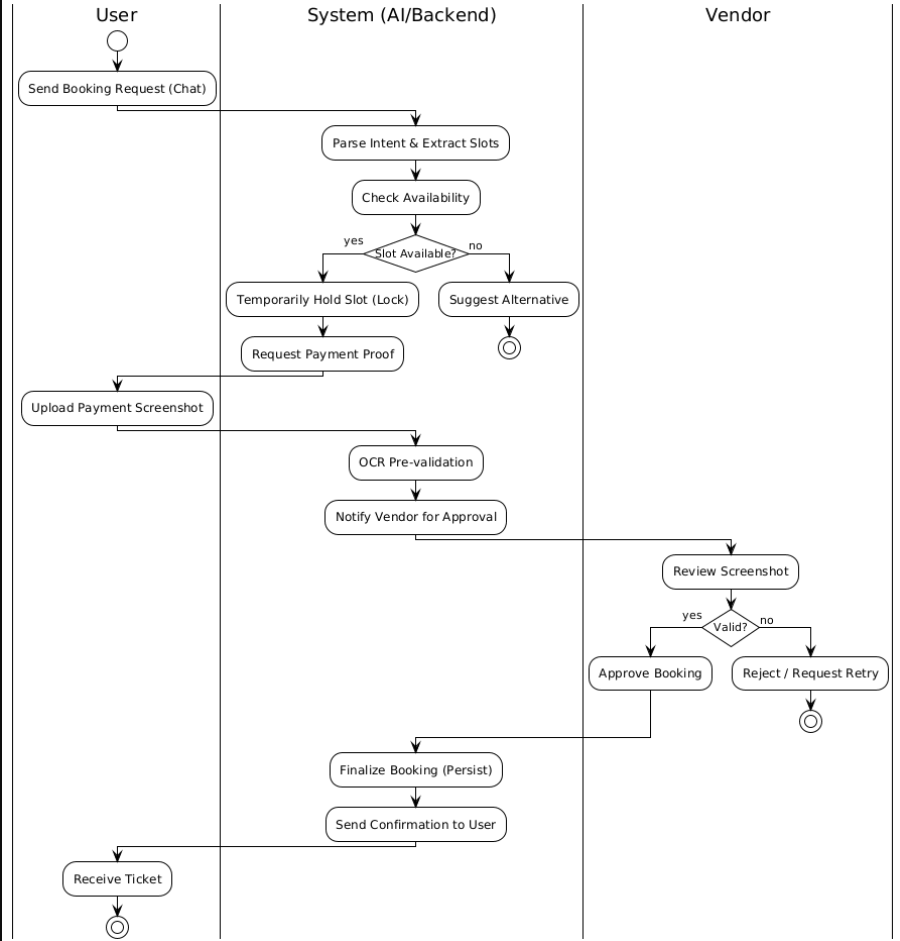
\includegraphics[width=0.95\textwidth]{images/Activity Diagram.png}
  }{
    \fbox{\parbox{0.85\textwidth}{\centering\vspace{0.8cm}
    Missing figure file: \texttt{images/Activity Diagram.png}\par
    Generic activity diagram placeholder\vspace{0.8cm}}}
  }
  \caption{General activity diagram of the booking lifecycle.}
  \label{fig:sds-general-activity}
\end{figure}

\subsubsection{Workflow 3: The Vendor Management Experience}

Vendors interact exclusively via the Vendor Dashboard.  Upon receiving a push
notification for a pending booking, the vendor views: customer name, service type,
requested date/time, advance payment amount, and the OCR-validated payment screenshot.
The vendor then taps Approve or Reject.  Approval triggers a Firestore write to
CONFIRMED and dispatches a WhatsApp confirmation to the customer.  Rejection triggers
a cascading slot release (AVAILABLE) and a WhatsApp rejection notice to the customer,
ensuring the system never deadlocks.

\begin{figure}[H]
  \centering
  \IfFileExists{images/FYP - Vend Activity Dig.png}{
    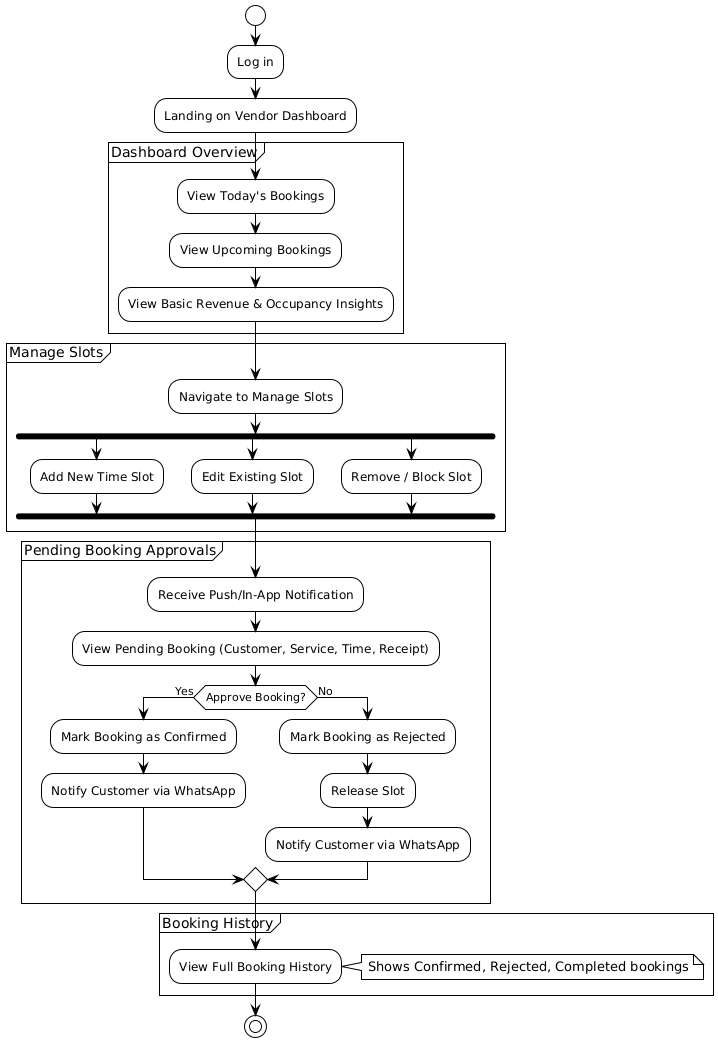
\includegraphics[width=0.95\textwidth]{images/FYP - Vend Activity Dig.png}
  }{
    \fbox{\parbox{0.85\textwidth}{\centering\vspace{0.8cm}
    Missing figure file: \texttt{images/FYP - Vend Activity Dig.png}\par
    Vendor activity diagram placeholder\vspace{0.8cm}}}
  }
  \caption{Vendor dashboard activity diagram for booking approval handling.}
  \label{fig:sds-vendor-activity}
\end{figure}

\begin{figure}[H]
  \centering
  \IfFileExists{images/FYP - Vend Activity Dig (1).png}{
    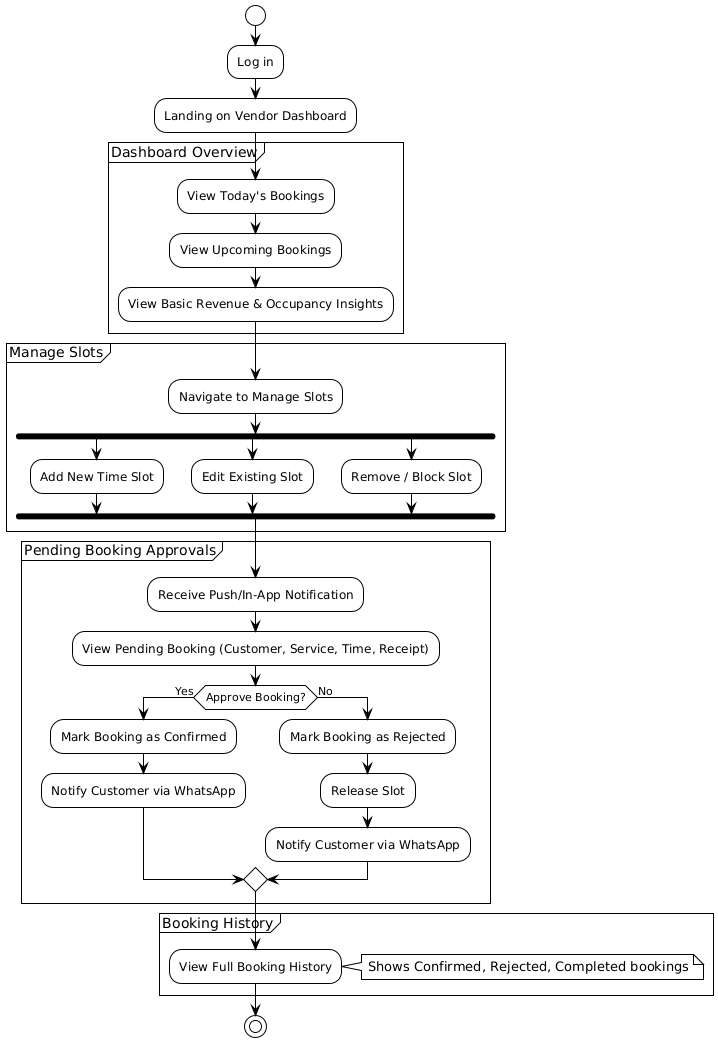
\includegraphics[width=0.95\textwidth]{images/FYP - Vend Activity Dig (1).png}
  }{
    \fbox{\parbox{0.85\textwidth}{\centering\vspace{0.8cm}
    Missing figure file: \texttt{images/FYP - Vend Activity Dig (1).png}\par
    Vendor activity diagram variant placeholder\vspace{0.8cm}}}
  }
  \caption{Vendor activity diagram variant for exception-handling paths.}
  \label{fig:sds-vendor-activity-alt}
\end{figure}

\subsection{Security Implementation}

\begin{description}
  \item[Authentication]
        Firebase Auth binds the secure \texttt{auth\_uid} token to all application
        data.  The API middleware validates ID tokens on every request.

  \item[Role-Based Access Control (RBAC)]
        Custom API middleware validates user claims (Vendor vs.\ Customer) before
        granting write access to critical Firestore collections (Services, Bookings,
        Approvals).

  \item[AI Guardrails (Prompt Injection Prevention)]
        The Neuro-Symbolic architecture means the LLM cannot issue database commands
        directly.  It classifies intent and extracts entities; all writes go through
        deterministic Python code nodes.  Malicious prompt injections attempting to
        bypass payment logic are structurally impossible.

  \item[Data Privacy]
        Payment screenshots are stored in a private Firebase Storage bucket.
        Time-limited Signed URLs are generated per-request and scoped to the specific
        vendor and admin only.  Screenshots are never publicly accessible.
\end{description}

%%% Local Variables:
%%% mode: latex
%%% TeX-master: "../report"
%%% End:
